%header and footer for separate chapter files

\ifx\whole\undefined
\documentclass[12pt, leqno]{book}
\usepackage{graphicx}
\input style-for-curves.sty
\usepackage{hyperref}
\usepackage{showkeys} %This shows the labels.
%\usepackage{SLAG,msribib,local}
%\usepackage{amsmath,amscd,amsthm,amssymb,amsxtra,latexsym,epsfig,epic,graphics}
%\usepackage[matrix,arrow,curve]{xy}
%\usepackage{graphicx}
%\usepackage{diagrams}
%
%%\usepackage{amsrefs}
%%%%%%%%%%%%%%%%%%%%%%%%%%%%%%%%%%%%%%%%%%
%%\textwidth16cm
%%\textheight20cm
%%\topmargin-2cm
%\oddsidemargin.8cm
%\evensidemargin1cm
%
%%%%%%Definitions
%\input preamble.tex
%\input style-for-curves.sty
%\def\TU{{\bf U}}
%\def\AA{{\mathbb A}}
%\def\BB{{\mathbb B}}
%\def\CC{{\mathbb C}}
%\def\QQ{{\mathbb Q}}
%\def\RR{{\mathbb R}}
%\def\facet{{\bf facet}}
%\def\image{{\rm image}}
%\def\cE{{\cal E}}
%\def\cF{{\cal F}}
%\def\cG{{\cal G}}
%\def\cH{{\cal H}}
%\def\cHom{{{\cal H}om}}
%\def\h{{\rm h}}
% \def\bs{{Boij-S\"oderberg{} }}
%
%\makeatletter
%\def\Ddots{\mathinner{\mkern1mu\raise\p@
%\vbox{\kern7\p@\hbox{.}}\mkern2mu
%\raise4\p@\hbox{.}\mkern2mu\raise7\p@\hbox{.}\mkern1mu}}
%\makeatother

%%
%\pagestyle{myheadings}

%\input style-for-curves.tex
%\documentclass{cambridge7A}
%\usepackage{hatcher_revised} 
%\usepackage{3264}
   
\errorcontextlines=1000
%\usepackage{makeidx}
\let\see\relax
\usepackage{makeidx}
\makeindex
% \index{word} in the doc; \index{variety!algebraic} gives variety, algebraic
% PUT a % after each \index{***}

\overfullrule=5pt
\catcode`\@\active
\def@{\mskip1.5mu} %produce a small space in math with an @

\title{Personalities of Curves}
\author{\copyright David Eisenbud and Joe Harris}
%%\includeonly{%
%0-intro,01-ChowRingDogma,02-FirstExamples,03-Grassmannians,04-GeneralGrassmannians
%,05-VectorBundlesAndChernClasses,06-LinesOnHypersurfaces,07-SingularElementsOfLinearSeries,
%08-ParameterSpaces,
%bib
%}

\date{\today}
%%\date{}
%\title{Curves}
%%{\normalsize ***Preliminary Version***}} 
%\author{David Eisenbud and Joe Harris }
%
%\begin{document}

\begin{document}
\maketitle

\pagenumbering{roman}
\setcounter{page}{5}
%\begin{5}
%\end{5}
\pagenumbering{arabic}
\tableofcontents
\fi


\chapter{Linear Systems}

Morphisms of a smooth curve $C$ (or indeed of any scheme) to a projective space are conveniently studied using the closely related notions of Divisors, linear systems and invertible sheaves. 

\section{Maps to projective space, and families of Cartier divisors}

Let $\phi: C\to \PP^{r}$ be a morphism from a smooth curve $C$. If $H\subset \PP^r$ is a hyperplane that does not contain $\phi(C)$, then the preimage of $\phi(C)\cap H$ is a finite sets of points on $C$, with multiplicities when $H$ is tangent to $\phi(C)$ or passes through a singular point of $\phi(C)$. Such a set of points with non-negative integer multiplicities is called an \emph{effective divisor} on $C$; more generally, a \emph{divisor} (sometimes called a \emph{Weil divisor})on a scheme $X$ is an integral linear combination of codimension 1 subvarieties, and it is called \emph{effective} if the coefficients are all non-negative. The divisors that arise as the pullbacks of general hyperplanes are special: since a hyperplane is defined by just one equation, which is locally given by the vanishing of a function, the pullback of a hyperplane will be locally defined by the vanishing of a single function that is a nonzerodivisor; that is, it is an  \emph{effective Cartier divisor}. See \cite[pp. 140-146]{H} for more information; on a smooth curve every divisor is Cartier, so the difference between Weil and Cartier divisors will not be an issue for us.) 

The  word ``local'' scattered through the previous paragraph is needed because, if $X$ is a projective variety, then the only algebraic functions $X\to \CC$ are constant functions. (Proof: the image of a projective variety
is again projective, and the only projective subvarieties of an affine variety are points.)

If we are given the family of divisors on $C$ that are the preimages of the intersections of hyperplanes with  $\phi(C)$, we can recover the map $\phi$ set-theoretically: it takes a point $p\in C$ to the point of projective space that is the intersection of those
hyperplanes whose preimages contain $p$. 

The relationship of two divisors on $C$ that are preimages of intersections of $\phi(C)$ with hyperplanes is simple to describe: If hyperplanes
$H, H'\subset \PP^r$ are defined by the linear form $h, h'$  then $1/h$ has a simple pole along $E$---we may say that it ``vanishes along $E$'' to degree $-1$.
In this sense the divisor $H-H'$ on $\PP^n$ is defined by the rational function $\lambda= h'/h$. If neither $H$ nor $H'$ contain $C$ then the pullback of $\lambda$ is a well-defined, nonzero rational function on $C$, and the divisor 
$\phi^{-1}(\phi(C)\cap H') - \phi^{-1}(\phi(C)\cap H)$ is defined by the pullback  $\phi^*(\lambda) := \lambda \circ f$. Thus the divisors arising from a given map to $\PP^{r}$ differ by the divisors of zeros minus poles of rational functions on $C$. 

If $C$ is a smooth curve then the local ring $\sO_{C,p}$ of $C$ at a point $p$ is a discrete valuation ring, and if $\pi$ is a generator of the maximal ideal of $\sO_{C,p}$, then any rational
function $\lambda$ on $C$ can be expressed uniquely as $u\pi^k$ where $u\in \sO_{C,p}$ is a unit and $k\in \ZZ$. We say that
the \emph{order} of $\lambda$ at $p$, and write $k = \ord_p \lambda$. We associate $\lambda$ to the divisor
$$
(\lambda) := \sum_{p\in C} (\ord_p\lambda)p.
$$
The \emph{class group} of $C$ is defined to be the the group of divisors on $C$ modulo the divisors of rational functions.
Thus the divisors on $C$ that are preimages of intersections of $\phi(C)$ with different hyperplanes all belong to the same
\emph{divisor class}, and form a linear system in the sense of the following section.

\section{Morphisms and linear systems}
We want to understand morphisms to $\PP^r$ more than set-theoretically, and we want to be able to produce them from data on $C$. For this we use the notion of linear system (sometimes called linear series). 

\begin{definition}
 A \emph{linear system} on a scheme $X$ is a pair $\sV  = (\sL, V)$ where $\sL$ is an invertible sheaf on $X$ and
 $V$ is a vector space of global sections of $\sL$. 
\end{definition}

We will spend the next pages unpacking this notion. Our goal is to explain and prove:
\begin{theorem}\label{maps and linear systems}
There is a natural bijection between the set of nondegenerate maps $\phi : C \to \PP^r$ modulo $PGL_{r+1}$, and basepoint-free linear systems of dimension $r$ on $C$.
\end{theorem}

Here ``nondegenerate" means the image of the map $\phi$ is not contained in any hyperplane. 



\subsection{Invertible sheaves}
Recall first that a \emph{coherent sheaf} $\sL$ on a scheme $X$ may be defined by
giving 
\begin{itemize}
 \item An open affine cover $\{U_{i}\}$ of $X$; 
 \item For each $i$, a finitely generated $\sO_{X}(U_{i})$-module $L_{i}$;
 \item For each $i,j$, an isomorphism $\sigma_{i,j}: L_{i}\mid_{U_{i}\cap U_{j}} \to L_{j}\mid_{U_{i}\cap U_{j}}$
 satisfying the compatibility conditions $\sigma_{j,k}\sigma_{i,j} = \sigma_{i,k}$. 
 \end{itemize}

A \emph{global section} of $\sL$ is a family of elements $t_{i}\in F_{i}$ such that 
$\sigma_{i,j} t_{i} = t_{j}$. Such a section may be realized as the image of the constant function 1 under
a homomorphism of sheaves $\sO_{X} \to \sL$. By Theorem \cite[Thm III.5.2]{H} the space $H^{0}(\sL)$  of global sections is
a finite-dimensional vector space. For example, $H^{0}(\sO_{X}) = \CC$ because the only globally defined
functions on $X$ are the constant functions.

The coherent sheaf $\sL$ is said to be an \emph{invertible sheaf} on $X$ if there is an open cover as above with the additional property
that $F_{i} \cong \sO_X(U_{i})$, the free module on one generator. 

If $\sigma \in H^0\sL$ is a global section of an invertible sheaf
on $X$, and $p\in X$ is a point, then $\sigma(p)$ is in the stalk of $\sL$ at $p$, a module isomorphic to $\sO_{X,p}$. Since the isomorphism is not canonical, $\sigma$ does not define a function on $X$ at $p$; but since any two isomorphisms
differ by a unit in $\sO_{X,p}$, the vanishing locus, denoted $(\sigma)_0$ of $\sigma$ \emph{is} a well-defined subscheme of $X$. Moreover, if $X$ is integral, then the ratio of two global sections is a well-defined rational function, so the divisor class of 
$(\sigma)_0$ is independent of the choice of $\sigma$.

\begin{proposition}
 The invertible sheaves on $X$ form a group under $\otimes_{X}$, called the 
\emph{Picard group of $X$}, denoted $\Pic(X)$. 
\end{proposition}
\begin{proof}
 If $\sF, \sG$ are invertible sheaves then so are $\sF\otimes_{X}\sG$ and  $\Hom_{X}(\sF, \sG)$, as one sees immediately by
restricting to the open sets where $\sF$ and $\sG$ are isomorphic to $\sO_{X}$. Moreover the natural isomorphisms
$$
\sF(U) \otimes_{X} \Hom(\sF(U), \sO_{X}(U)) \to \sO_{X}(U)\quad s \otimes f \mapsto f(s)
$$ 
patch together to define a global isomorphism 
$$
\sF \otimes_{X} \Hom(\sF, \sO_{X}) \to \sO_{X}
$$
justifying the definition
$\sF^{-1} := \Hom(\sF, \sO_{X})$ and thus the name ``invertible sheaf''. 
\end{proof}
 
If $D\subset X$ is an effective divisor, then we define $\sO_{X}(-D)$ to be the ideal sheaf of $D$. If $D$ is locally defined by the vanishing of a (locally defined) nonzerodivisor in $\sO_{X}$, (that is, $D$ is a Cartier divisor), then
$\sO_{X}(-D)$ is an invertible
sheaf.
We write $\sO_{X}(D)$ for the inverse, $\sO_{X}(-D)^{-1}$. The dual of the inclusion
$\sO_{X}(-D)\subset \sO_{X}$ is a map $\sO_{X} \to \sO_{X}(D)$ sending the global section $1\in \sO_{X}$ to a section
$\sigma\in \sO_{X}(D)$ that vanishes precisely on $D$.

\begin{example} [Invertible sheaves on $\PP^{r}$]\label{linear systems on Pr} If $H\subset \PP^{r}$ is a hyperplane defined by the vanishing of a linear form $\ell = \ell(x_{0}, \dots x_{r})$ then the ideal sheaf $\sO_{\PP^{r}}(-1) := \sI_{H/\PP^{r}}\subset \sO_{\PP^{r}}$ is generated on the open affine set 
$U_{i}:= \{x_{i}\neq 0\} \cong \AA^{r}$
by $\ell/x_{i}$, and is thus an invertible sheaf. 
Moreover, if $H'$ is the hyperplane defined by another linear form $\ell'$, then 
$$
\frac{\ell'}{\ell}\cdot\sI_{H/\PP^{r}} = \sI_{H'/\PP^{r}} 
$$
\fix{check that this is out notation for ideal sheaf}
so the sheaves $\sI_{H/\PP^{r}}$ and $\sI_{H'/\PP^{r}} $ are isomorphic, justifying the name $\sO_{\PP^{r}}(-1)$.

The $p$-th tensor power of $\sO_{\PP^{r}}(-1)$ is called $\sO_{\PP^{r}}(-d)$; it is isomorphic to the
ideal sheaf of any hypersurface of degree $d$. Because polynomials satisfy the unique factorization property,
every effective divisor $D\subset \PP^{r}$ is a hypersurface of some degree $d$, so
$\sO_{\PP^{r}}(-D) \cong \sO_{\PP^{r}}(-d)$. Note that if $d>0$ then $H^{0}(\sO_{\PP^{r}}(-D)) = 0$, since it may be realized
as the sheaf of locally defined functions vanishing on $D$, and there are no such
globally defined functions except 0.

We take $\sO_{\PP^{r}}(d)$ to be the inverse of $\sO_{\PP^{r}}(-d)$. If $D$ is the hypersurface defined by 
a form $F$ of degree $d$, then $\sO_{\PP^{r}}(-D)$ is generated on $U_{i}$ by $F/(x_{i}^{d})$, so
$\sO_{\PP^{r}}(D)$ is generated on $U_{i}$ by $x_{i}^{d}/F$.
Starting from the inclusion 
$
\sO_{\PP^{r}}(-D) \subset \sO_{\PP^{r}}
$
and taking inverses, we see that 
$
\sO_{\PP^{r}} \subset \sO_{\PP^{r}}(D)
$
and the global section $1\in H^0(\sO_{\PP^{r}})\subset H^0(\sO_{\PP^{r}}(D))$, restricted to
$U_{i}$, is $F/(x_{0}^{d})$ times the local generator of $\sO_{\PP^{r}}(D)$ and thus vanishes on $D$.
 Because every
rational function on $\PP^{r}$ has degree 0, and any two global sections differ by a rational
function, it follows that every global section of $\sO_{\PP^{r}}(d)$ vanishes on a divisor of degree $d$. Thus
we may identify $H^{0}(\sO_{\PP^{r}}(d))$ with the ${n+d\choose n}$-dimensional vector space of forms of degree $d$ on $\PP^{r}$.
\end{example}

The proof of Theorem~\ref{maps and linear systems} is contained in the material of the next two subsections:

\subsection{The map to projective space coming from a linear system} 
For any $\CC$-vector space $V$ of dimension $r+1$ with basis $x_{0}, \dots, x_{r}$, we write $\Sym(V) \cong \CC[x_{0},\dots, x_{r}]$ for the symmetric algebra on $V$, and
$\PP(V)\cong \PP^{r}_{\CC}$ to be the projective space ${\rm Proj}(\Sym(V))$, which is naturally isomorphic to the
space of lines in $V^{*}$. Note that the isomorphism $\PP(V)\cong \PP^{r}_{\CC}$ is well-defined up to the action
of $\Aut(\PP^r) = PGL(r+1)$.


Given a linear system $\sV:=(\sL, V)$  of dimension $r$ on a scheme $X$, where
$\sL$ is an invertible sheaf on $X$ and $V = \langle\sigma_{0}, \dots \sigma_{r}\rangle$ is a vector space of global sections, we define the \emph{base locus} of $\sV$ to be the closed subscheme 
$$
B_\sV := \bigcap_{i= 0}^{r}\{\sigma_{i} = 0\}.
$$
Let $W:=X\setminus B_\sV$ be the open subscheme where not all sections $\sigma_{i}$ vanish.

For any point $q\in W$ we  may choose an open neighborhood $W'\subset W$ of $q$, and an identification 
$$
t: \sL\mid_{W'} \rTo^{\cong} \sO_{W'}
$$
and define $\phi_{\sV}: W' \to \PP(V)$ by 
$$
W'\ni p \mapsto \bigl(t(\sigma_{0}(p)),\dots, t(\sigma_{r}(p))\bigr) \in \PP(V).
$$
This map is obviously a morphism on $W'$. A change of neighborhoods $W'$ or of identifications $t$ would multiply
each value $t(\sigma_{i}(p))$ by a unit, the same one for each $i$, and thus the construction would define the same morphism. It follows that the morphisms
defined on different $W'$ agree on overlaps, and thus define a morphism $W \to \PP(V) \cong \PP^r$. This is the reason
that the dimension of $\sV$ is defined to be $r=\dim V -1$ instead of $\dim V$.

The most useful linear series are those that define morphisms defined on all of $X$. This happens when $B_\sV = \emptyset$,
that is, for every point $q\in X$, there is a section $\sigma \in V$ such that $\sigma$ does not vanish at $x$. In this case we say that $(\sL, \sV)$ is \emph{basepoint free}.

\subsection{The linear system coming from a map to projective space}

Conversely, suppose that we are given a morphism $\phi: X\to \PP^{r}$. With notation as in Example~\ref{linear systems on Pr} we may choose an open affine cover $W_{i,j}$ of $X$ such that $\phi(W_{i,j})\subset U_{j}$. Composing the regular
functions
$x_{0}/x_{j},\dots, x_{r}/x_{j}$ with $\phi$ we get functions $\sigma_{0},\dots,\sigma_{r}$ on $W_{i,j}$.  The function $\sigma_{j}$, is the image under $\phi^*: \sO_{U_j} \to \sO_{W_{i,j}}$ of the function $x_j/x_j = 1$ on $U_{j}$, so it $\sigma_j = 1\in \sO_{W_{i,j}}$. In particular, the module $\sL_{\phi^{-1}(U_j)}$ generated by the rational functions 
$$
\{(\sigma_i)_{\phi^{-1}(U_j)} = \phi^*(x_i/x_j)\}_{0\leq i\leq n}
$$
 is a free $\sO_{W_{i,j}}$-module on 1 generator. On the preimage of $U_j\cap U_k$ these sections differ by the common unit $\phi^*(x_k/x_j)$, and thus the collection of these modules defines an invertible sheaf $\sL$ on $X$ together with an
$r+1$-dimensional space of global sections $\sV := \langle \sigma_0,\dots \sigma_r\rangle$ that forms a basepoint free linear system. Note that the subscheme  $\{\sigma_k = 0\} \subset W_{i,j}$  is the scheme-theoretic preimage of the
the hyperplane $\{x_k = 0\}\subset \PP^r$. This completes the explanation and proof of Theorem~\ref{maps and linear systems}


\subsection{More about linear systems}
Let $\sV = (\sL, V)$ be a linear sysytem on $X$.  The linear system is said to be \emph{complete} if $V = H^0(\cL)$; in this case it is sometimes denoted $|\cL|$. If $\cL \cong \cO_C(D))$, we also write it as $|D|$. 
The \emph{dimension of $\sV$} is $\dim V -1$ . If $D$ is any divisor on $C$ we write $r(D)$ for the dimension of the complete linear series $|D|$; that is, $r(D) = h^0(\cO_C(D)) - 1$. Finally, a linear system of dimension 1 is called a \emph{pencil}, a linear system of dimension 2 is called a \emph{net} and, less commonly, a three-dimensional linear system is called a \emph{web}.


Via the correspondence of Theorem~\ref{maps and linear systems}, the statements about the geometry of a map $\phi : C \to \PP^r$ can be formulated as statements about the relevant linear systems. We will see this in many instances throughout this book. Here is a first example:

\begin{proposition}\label{very ample}\cite[Thm. IV.3.1]{H}
Let $\cL$ be an invertible sheaf on a smooth curve $C$. The complete linear system $|\cL|$ is base-point-free iff
$$
h^0(\cL(-p)) = h^0(\cL) - 1 \quad \forall p \in C;
$$
and in this case the associated map $\phi_\cL$ is an embedding iff
$$
h^0(\cL(-p-q)) = h^0(\cL) - 2 \quad \forall p, q \in C.
$$
\end{proposition} 

\begin{proof}
The statement $h^0(\cL(-p-q)) = h^0(\cL) - 2$ for $p \neq q$ implies that $\phi_\cL(p) \neq \phi_\cL(q)$. The tangent space of $C$ at $p$ is $(\sI_C(p)/\sI_C(p)^2)^*$, so the condition that there is a section of $\sL$ that vanishes at $p$, but does not vanish
to order 2, implies that the differential $d\phi_\cL$ is injective at $p$.
\end{proof}

We can also relate the geometry of the map associated to a incomplete linear system $V \subset H^0(\cL)$ to the geometry of the map associated to the complete linear system $|\cL|$. In general, if $V \subset W \subset H^0(\cL)$ are a pair of nested linear systems, we have a linear map $W^* \to V^*$ dual to the inclusion $V \hookrightarrow W$, and a corresponding linear projection $\pi : \PP W^* \dashrightarrow \PP V^*$, with indeterminacy locus the subspace $\PP(Ann(V)) \subset \PP W^*$. In this case, we have 
$$
\phi_V = \pi \circ \phi_W;
$$
that is, we have the diagram 

\begin{diagram}
& & \PP W^* \\
& \ruTo^{\phi_W} & \dDashto_\pi \\
C & \rTo^{\phi_V} & \PP V^*.
\end{diagram}

Note that in this case, given that $W$ is base-point-free, the condition that $V$ be base-point-free is equivalent to saying that the center $\PP(Ann(V))$ of the projection map $\pi$ is disjoint from $\phi_W(C)$.

By way of language, we will say that a curve $C \subset \PP^r$ embedded by a complete linear series is \emph{linearly normal}; this is equivalent to saying that the restriction map
$$
H^0(\cO_{\PP^r}(1)) \to H^0(\cO_{C}(1))
$$
is surjective, which is in turn equivalent to saying that $C$ is not the regular  projection of a nondegenerate curve $\tilde C \subset \PP^{r+1}$.

\begin{exercise}
Extend the statement of Proposition~\ref{very ample} to incomplete linear systems; that is, prove that the map associated to a linear system $(\cL, V)$ is an embedding iff
$$
\dim\big( V \cap H^0(\cL(-p-q))\big) = \dim V - 2 \quad \forall p, q \in C.
$$
\end{exercise}

\begin{exercise}
An automorphism of $\PP^r$ takes hyperplanes to hyperplanes. Deduce that it is given by the linear system
$\sV = \sO_{\PP^r}(1), H^0(\sO_{\PP^r}(1))$, and use this to show that $\Aut \PP^r = PGL(r+1)$. 
\end{exercise}

\begin{exercise}
Show that, if $s<r$, then the image of any morphism $\PP^r \to \PP^s$ is a single point.
\end{exercise}

For another example of the relationship between linear series on curves and maps of curves to projective space, consider a smooth curve $C \subset \PP^r$ embedded in projective space, and assume that $C$ is linearly normal. If $\phi : C \to C$ is any automorphism, we can ask whether $\phi$ is induced by an automorphism of $\PP^r$; in other words, does there exist an automorphism $\Phi : \PP^r \to \PP^r$ such that $\Phi(C) = C$ and $\Phi|_C = \phi$? The answer is expressed in the following exercise.

\begin{exercise}\label{projective automorphism}
In the circumstances above, the automorphism $\phi$ is induced by an automorphism of $\PP^r$ if and only if $\phi$ carries the invertible sheaf $\cO_{C}(1)$ to itself; that is, $\phi^*(\cO_{C}(1)) = \cO_{C}(1)$.
\end{exercise}

For example, consider the image of $\PP^1$ in $\PP^n$ under the map given by the complete linear system $|\cO_{\PP^1}(n)|$; this is called the \emph{rational normal curve}. Since there is a unique invertible sheaf of each degree $n$ on $C$, and the curve is linearly normal, we see that \emph{every automorphism of a rational normal curve $C \subset \PP^n$  is projective}.

If $\sL, \sL'$ are linear systems on a smooth curve $C$ and $D = (\sigma)_0,D' = (\sigma')_0$ are the divisors of zeros of sections of $\sL$ and $\sL'$ respectively, then $D+D'$ is the divisor of zeros of the section $\sigma\otimes \sigma'$ of
$\sL\otimes \sL'$.

We  often want to consider sections of a given invertible sheaf $\cL$ with bounded singularities: if $D = \sum m_ip_i$ is a divisor, we define the invertible sheaf $\cL(D)$ to be the sheaf of rational sections $\sigma$ of $\cL$ satisfying $\ord_{p_i}(\sigma) \geq -m_i$ for all $i$; as a line bundle, this is the same as $\cL \otimes \cO_C(D)$.

If $\phi:X \to \PP^r$ is a generically finite morphism, then the \emph{degree of $\phi$} is the number of points in the preimage of a general point of $\phi(X)$. Thus, for example, if $D := \sum_{p\in C} n_pp$ is a divisor on a smooth curve, and the linear system $|D|$ is basepoint free, then the degree of the map associated to $|D|$ is $\deg D := \sum_{p\in C} n_p$.

\subsection{The most interesting linear system}

The most important invertible sheaf on a smooth curve $C$ is the sheaf of global sections of the cotangent bundle of $C$, called the canonical sheaf $\omega_C$ of $C$ (for canonical sheaves more generally, see Chapter~\ref{dualizing sheaf}). A section of 
$\omega_C$ is thus a globally defined differential form (also called a 1-form) on $C$, and the divisor class
of such a form is usually denoted $K_C$. The importance of the canonical sheaf is made clear by the results of the next section.


\section{Genus, Riemann-Roch and Serre Duality}

We will henceforward assume that the reader is acquainted with sheaf cohomology (at least sufficiently to write
$H^i(X; \sF)$ or (our preferred form) $H^i(\F)$ without blushing). If $D$ is a divisor on a scheme $X$ we will often
abbreviate $H^i(\sO_X(D))$ to $H^i(D)$, and *** h^i***

\subsection{The genus of a curve}

Any discussion of the geometry of smooth projective curves has to start with the notion of the \emph{genus} of a curve, the sole topological invariant. The most natural and intuitive definition is topological: if $C \subset \PP^r$ is a smooth curve, we can think of it as a submanifold of the complex projective space $\PP^r(\CC)$ with the classical topology; as such, it is a compact, oriented surface, and so its topological type is described by its topological genus---informally, the ``number of holes."

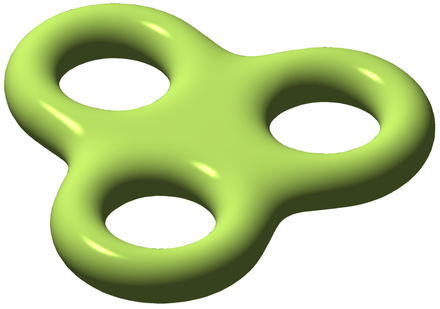
\includegraphics[scale = 1]{RiemannSurface}
**** Riemann Surface of genus 3, from Wikimedia ****

Of course this definition does not apply to curves over fields other than $\CC$, and doesn't relate the genus to the algebra of the curve. However, we can relate the topological genus of a curve directly to its topological Euler characteristic: we have
$$
g(C) = 1 - \frac{\chi_{top}(C)}{2}.
$$
At the same time, by the Hopf index theorem, the topological Euler characteristic is the degree of the tangent sheaf, which, because $C$ is 1-dimensional as a complex manifold, is the dual of the canonical sheaf; thus
$$
g(C) = \frac{\deg(K_C)}{2} + 1,
$$
which we adopt as the definition of $g(C)$.

Other characterizations of the genus require more machinery to establish. We will give some here, and use  tools from the following section to prove equivalence.

\begin{enumerate}

\item\label{genus 1forms} $g(C)$ is the dimension of the vector space of regular 1-forms (that is, global sections of the
cotangent sheaf) on $C$.

\item The Euler characteristic of the structure sheaf of $C$ is $\chi(\cO_C) = h^0(\cO_C) - h^1(\cO_C)$. Since $h^0(\cO_C) = 1$, 
$$
g(C) = 1 - \chi(\cO_C).
$$

\item\label{genus Hilbert} If $C \subset \PP^r$ is embedded as a curve of degree $d$, with homogeneous coordinate ring
$S_C$, then the function $d \mapsto \dim_\CC (S_C)_d$ is equal to a polynomial function $p_C(m)$ for large $d$. We have:
$$
p_C(m) =  dm - g + 1,
$$
so $g(C) = 1 - p_C(0)$. 
\end{enumerate}

\subsection{The Riemann-Roch Theorem}

To prove that the formula's for the genus given above are correct, we use the \trr and Serre duality (sometimes called Kodaira-Serre duality, since Kodaira was responsible for the analytic version.)

\begin{theorem}[Riemann-Roch Theorem]\label{RR}
 If $C$ is a smooth, connected projective curve of genus $g$, and $D$ a divisor of degree $d$ on $C$, it says that
$$
h^0(D) = d - g + 1 + h^0(K_C - D).
$$
\end{theorem}

For example, if we take $D=0$, this tells us that $h^0(K) = g$, proving the characterization~(\ref{genus 1forms}) above. Also, since $h^0(D) = 0$ for any divisor $D$ of negative degree, we have:

\begin{corollary}\label{nonspecial RR}
For any divisor of degree $d \geq 2g-1$, we have
$$
h^0(D) = d - g + 1.
$$
\end{corollary}

Using this, we can apply Proposition~\ref{very ample} to characterize the linear series that give embeddings:

\begin{corollary}\label{degree 2g+1 embedding}
Let $D$ be a divisor of degree $d$ on a smooth, connected projective curve of genus $g$. If $d \geq 2g$, the complete linear series $|D|$ is base point free; and if $d \geq 2g+1$ the associated map $\phi_D : C \to \PP^{d-g}$ is an embedding.
\end{corollary}

Since the complement of a hyperplane in projective space is an affine space, we get an affine embedding result too:

\begin{corollary}
 If $C$ is any smooth, connected projective curve and $\emptyset \neq \Gamma \subset C$ a finite subset then $C \setminus \Gamma$ is affine.
\end{corollary}
\begin{proof}
Let $D$ be the divisor defined by $\Gamma$ By Corollary~\ref{degree 2g+1 embedding} a high multiple of $D$ is very ample,
and gives an embedding $\phi: C\to \PP^n$ such that the preimage of the intersection of $C$ with some hyperplane $H$
is a multiple of $D$. It follows that $C\setminus \Gamma$ is embedded in $\PP^n\setminus H$.
\end{proof}


We can  use \TRR in the simple case of Corollary~\ref{nonspecial RR} to determine the Hilbert polynomial of a projective curve. To do this, let $C \subset \PP^r$ be a smooth curve of degree $d$ and genus $g$, and consider the exact sequence of sheaves
$$
0 \rTo \cI_{C/\PP^r}(m) \rTo \cO_{\PP^r}(m) \rTo \cO_C(m) \rTo 0
$$
and the corresponding exact sequence
$$
 H^0(\cO_{\PP^r}(m)) \rTo^{\rho_m} H^0(\cO_C(m)) \rTo H^1(\cI_{C/\PP^r}(m)) \rTo 0.
$$
The \emph{Hilbert function} $h_C$ of $C$  is defined by
$$
h_C(m) = \rank(\rho_m);
$$
 since $H^1(\cI_{C/\PP^r}(m)) = 0$ for large $m$, this is equal to $h^0(\cO_C(m))$, which by Riemann Roch equals $md-g+1$, again for large $m$. Thus, the Hilbert polynomial of $C \subset \PP^r$ is $p_C(m) = dm-g+1$, establishing the characterization~(\ref{genus Hilbert}) above.
 
 Note that the Riemann-Roch formula does not give us a formula for the dimension $h^0(D)$ when $h^0(K_C - D)>0$; such divisors $D$ are called \emph{special divisors}, or \emph{special divisor classes}. 
 
 
\begin{fact}
 Classically, the dimension $h^0(K_C-D) = h^1(D)$ was called the \emph{superabundance} of $D$: the idea was that a divisor of degree $d$ had, at a minimum, $d-g+1$ sections and $h^1(D)$ represented the number of ``extra " sections. Even though the introduction of cohomology was still almost a century away, the ranks of cohomology groups $h^1$ had classical names, often involving the term superabundance---a premonition of the Riemann-Roch theorem in general.
\end{fact}
 
\begin{fact}
If $k$ is a field that is not algebraically closed there may be genus 0 curves that are not isomorphic to $\PP^1$. However, they must be``forms'' of $\PP^1$ in the sense that they become isomorphic to $\PP^1$ after extension of scalars to 
the algebraic closure $\overline k$ of $k$. The unique example with $k = \RR$ is the conic $x^2+y^2+z^2 = 0$. Indeed, any form of $\PP^1$ over any field $k$ can all be embedded in $\PP_{k}^2$ (by using the anti-canonical linear system.

The curve $\PP_k^1$ itself may be described as the scheme of left ideals of $k$-vector-space dimension 1 in the ring of
$2\times 2$ matrices over $k$ (such an ideal can be embedded in the matrix ring as a linear combination of the 2 columns in an appropriate sense). More generally, any scheme that is a form of $\PP^1$ over $k$
may be described as the scheme of 1-dimensional left ideals in a central simple ($=$ Azumaya) algebra over $k$---though as a set this scheme has no $k$-rational points unless the algebra is the algebra of $2\times 2$ matrices!
\end{fact}
\subsection{Serre duality}

In general, if $\cF$ and $\cG$ are coherent sheaves on a scheme $X$, we have for every $i$ and $j$ a cup product map
$$
H^i(\cF) \otimes H^j(\cG) \to H^{i+j}(\cF \otimes \cG).
$$

Suppose now that $C$ is a smooth, projective curve, and that $D$ is any divisor on $C$. 

\begin{theorem}[Serre Duality]\label{sd} Let $C$ be a smooth connected projective curves with canonical divisor $K$. We have
 $$
h^1(K) = 1
$$
and the cup product map
$$
H^1(D) \otimes H^0(K-D) \to H^1(K)
$$
is a perfect pairing; that is, it induces a natural isomorphism
$$
H^1(D) = H^0(K-D)^*.
$$
\end{theorem}

\subsection{A partial proof}

Combining \TRR and Serre Duality we get:
\begin{corollary}
 If $C$ is a smooth, connected projective curve and $D$ is a divisor on $C$ then
\end{corollary}
$$
\chi(\sO_C(C)) := h^0(D) - h^1(D) = d-g+1
$$
or in other words, for any invertible sheaf $\cL$ of degree $d$ on $C$,
$$
\chi(\cL) = d-g+1
$$
which is pretty easy to prove. To see this, observe that for any invertible sheaf $\cL$ on $C$ and any point $p \in C$ we have an exact sequence of sheaves
$$
0 \to \cL(-p) \to \cL \to \cL_p \to 0.
$$
It follows that $\chi(\cL(-p)) = \chi(\cL) - 1$, so that Riemann-Roch for $\cL$ is equivalent to Riemann-Roch for $\cL(-p)$. Since any divisor can be obtained from 0 by adding and subtracting points, the Riemann-Roch formula for an arbitrary $\cL$ follows from the special case $\cL = \cO_C$.


\section{The canonical map}

Given the central role played by the canonical divisor class, it is natural to look at the geometry of the map $\phi_K : C \to \PP^{g-1}$ associated to the complete canonical series $|K|$. To do this, we first have to single out a special class of curves:

\begin{definition}
A curve $C$ of genus $g \geq 2$ is said to be \emph{hyperelliptic} if there exists a map $f : C \to \PP^1$ of degree 2; equivalently, if there exists a invertible sheaf $\cL$ on $C$ of degree 2 with $h^0(\cL) = 2$.
\end{definition}

The basic theorem about the canonical map is then

\begin{proposition}
Let $C$ be a smooth, projective curve of genus $g\geq 2$. The canonical map $\phi_K : C \to \PP^{g-1}$ is an embedding if and only if $C$ is not hyperelliptic.
\end{proposition}

\begin{proof}
This is just a direct application of Proposition~\ref{very ample} to the Riemann-Roch formula. To see that $\phi_K$ is an embedding, we have to show that for any pair of points $p, q \in C$ we have
$$
h^0(K_C(-p-q)) = h^0(K_C)-2 = g-2.
$$
Applying Riemann-Roch, we see that this is the case if and only if $h^0(\cO_C(p+q)) = 1$ for any $p,q \in C$, which is the case if and only if $C$ is not hyperelliptic.
\end{proof}

Note that if $C$ is hyperelliptic, the map $\phi_K$ factors through the degree 2 map $\pi : C \to \PP^1$: if $\{p,q\} \subset C$ is a fiber of this map, we have $h^0(\cO_C(p+q)) = 2$ and hence $\phi_K(p) = \phi_K(q)$. The image of the map $\phi_K$ is a nondegenerate curve of degree $g-1$ in $\PP^{g-1}$, which we will see is a \emph{rational normal curve}. This observation implies in particular that if $C$ is hyperelliptic of genus $g \geq 2$, then the invertible sheaf $\cL$ of degree 2 with $h^0(\cL) = 2$ is in fact unique.

Hyperelliptic curves are very special, at least when $g \geq 3$ (in case $g=2$ the canonical map itself is a degree 2 map $C \to \PP^1$; all curves of genus 2 are hyperelliptic): in the family of all curves, as we'll see, they comprise a closed subvariety. In particular, the behavior of linear series and maps on a hyperelliptic curve is very different from that of series on a general curve; when we discuss the geometry of curves of low genus in the Chapter~\ref{}, we will exclude  the hyperelliptic case, and deal with this case in a separate chapter.

For non-hyperelliptic curves, however, the geometry of the canonical map, and its image, the canonical curve, are the keys to understanding the curve. We'll see this in detail in many cases in the following chapter; for now, we mention one highly useful result along these lines.

\fix{add here: canonical series on plane curves cut by $|\cO_{\PP^2}(d-3)|$; consequence that no smooth plane curve can be hyperelliptic}

\fix{maybe move initial discussion of hyperelliptic curves from Ch. 6 to a section here}

\fix{also add to this chapter: differentials on plane curves $C$, possibly with nodes or more general singularities; adjoint conditions; algorithm for determining the complete linear system associated to a divisor $D$ on $C$}

\subsection{The geometric Riemann-Roch theorem}

Let's state this first in a relatively simple case: let $C$ be a nonhyperelliptic curve, embedded in $\PP^{g-1}$ by its canonical series and let $D = p_1+\dots + p_d$ be a divisor consisting of $d$ distinct points; let $\overline D$ be the span of the points $p_i \in C \subset \PP^{g-1}$. Since the hyperplanes in $\PP^{g-1}$ containing $\{p_1,\dots,p_d\}$ correspond (up to scalars) to sections of $K_C$ vanishing at the points $p_1$, we see that
$$
h^0(K_C-D) = g - 1 - \dim \overline D.
$$
Plugging this into the Riemann-Roch formula, we arrive at the statement
$$
r(D) = d - 1 - \dim \overline D;
$$
or in other words, \emph{the dimension of the linear series $|D|$ in which the divisor $D$ moves is equal to the number of linear relations on the points $p_i$ on the canonical curve}. Thus, for example, if $D = p_1+p_2+p_3$, we see that $D$ moves in a pencil if and only if the points $p_i$ are collinear.

We can extend this statement to the case of arbitrary effectived divisors $D$ (and even hyperelliptic curves) if we define our terms correctly. To do this, suppose $f : C \to \PP^d$ is any map, and $D \subset C$ any divisor. We define the \emph{span} of the divisor $D$ under the map $f$ to be the intersection
$$
\overline{f(D)} = \bigcap_{H \mid f^{-1}(H)\supset D} H 
$$
of all hyperplanes in $\PP^d$ whose inverse image in $C$ contains $D$. In these terms, we can state the \emph{geometric Riemann-Roch} as

\begin{theorem}
If $C$ is any curve of genus $g \geq 2$,  $\phi : C \to \PP^{g-1}$ its canonical map and $D \subset C$ any effective divisor of degree $d$, then
$$
r(D) = d - 1 - \dim \overline{\phi(D)}.
$$
\end{theorem}

 \section{The Riemann-Hurwitz formula}
 
 The Riemann-Hurwitz formula does a simple thing: given a (nonconstant) map $f : C \to X$ of smooth projective curves, it relates the genera of $C$ and $X$ via the geometry of the map. The proof is likewise simple.
 
 To set it up, we first introduce the notion of \emph{ramification} of such a map. Suppose $p \in C$ is any point, with $q = f(p) \in X$ its image in $X$. In terms of a suitable choice of local coordinates $z$ on $C$ around $p$ and $w$ on $X$ around $q$, we can write the map simply as $z \mapsto w = z^m$ for some integer $m > 0$; the integer $m-1$ is then called the \emph{ramification index} of $f$ at $p$, and denoted $\ram(f,p)$. To characterize this without invoking local coordinates, we can say that for any point $q \in X$ we have
 $$
 f^{-1}(q) = \sum_{p\in C \mid f(p)=q} (\ram(f,p)+1)\cdot p
 $$
 as subschemes (or, equivalently, divisors) on $C$. The \emph{ramification divisor} of $f$ is defined to be the divisor
 $$
 R = \sum_{p \in C} \ram(f,p)\cdot p \; \in \;  \Div(C);
 $$
 the \emph{branch divisor} is the corresponding divisor
 $$
 B = \sum_{q \in X} \Big(\sum_{p \in f^{-1}(q)} \ram(f,p) \Big)\cdot q \; \in \; \Div(X).
 $$
 Note that $R$ and $B$ have the same degree $\sum_{p \in C} \ram(f,p)$. Note also that just to define the divisor $R$ requires we know that \emph{not every point of $C$ is a ramification point}; that is, $\ram(f,p) = 0$ at a general point $p \in C$, which may be false in characteristic $p > 0$; thus the argument sketched here requires the hypothesis of characteristic 0.
 
 To relate the genera of $X$ and $C$ in this situation, start by choosing any rational 1-form $\omega$ on $X$; let $\eta = f^*(\omega)$ be its pullback to $C$. For simplicity, we will assume that the zeroes and poles of $\omega$ lie outside the branch divisor $B$, so that $\omega$ will be regular and nonzero at each branch point. (We can certainly find such a form, and in any event the calculation goes through without this assumption, albeit with more complicated notation.) We know that $\deg(\omega) = 2g(B) - 2$ and $\deg(\eta) = 2g(C) - 2$; we will relate these two by describing the zeroes and poles of $\eta$ in terms of those of $\omega$.
 
 First of all, since the zeroes of $\omega$ lie outside the branch divisor $B$, for every zero of $\omega$ of multiplicity $m$ we have exactly $d$ zeroes of $\eta$, each with multiplicity $m$; and likewise for the poles of $\omega$. Meanwhile, at every point of $B$ the form $\omega$ is regular and nonzero; and by the description of the map $f$ in terms of local coordinates we see that $\eta$ will have a zero of multiplicity $\ram(f,p)$ at every point $p \in R$. In sum, then, we have
 $$
 \deg((\eta)) = d\cdot \deg((\omega)) + \sum_{p \in C} \ram(f,p) \cdot p,
 $$
 or in other words,
 $$
 2g(C) - 2 = d(2g(X)-2) + \deg R;
  $$
  this is the Riemann-Hurwitz formula. Note that if the target curve $X \cong \PP^1$ has genus 0, the formula reads
  $$
  g(C) = -d  + 1+ \frac{\deg R}{2}
  $$
 or equivalently
 $$
 \deg R = \deg B  = 2d + 2g(C) - 2.
 $$
 
 \subsection{An application}
 
 Let $V$ be the vector space of homogeneous polynomials of degree $d$ in two variables; that is, $V = H^0(\cO_{\PP^1}(d))$. In the projectivization $\PP V \cong \PP^d$, let $\Delta$ be the locus of polynomials with a repeated factor. It's not hard to see that $\Delta$ in a hypersurface; we ask, what is its degree?
 
 To answer this, let $L \subset \PP V$ be a general line---that is, a general pencil of divisors of degree $d$ on $\PP^1$. The linear system $L$ defines a map $\phi_L : \PP^1 \to \PP^1$ of degree $d$, and the locus $L \cap \Delta$ is exactly the branch divisor $B$.
 It follows then that
 $$
 \deg(\Delta) = \deg(L \cap \Delta) = \deg B = 2d-2,
 $$
 answering our question. Note that since $L$ is general, both $L\cap \Delta$ and $B$ are reduced divisors, so we can interpret the above simply as an equality of cardinality of sets; but if we keep track of multiplicities the argument goes through for an arbitrary $L \not\subset \Delta \subset \PP^d$.
 
 \section{Hyperelliptic Curves}
 
 
 This will be a somewhat anomalous section, in keeping with its subject matter. In the world of curves, hyperelliptic curves are outliers: they behave differently from other curves, and the techniques used to analyze them are correspondingly different from how we approach more general curves. As you'll see in following chapters, many theorems about curves contain the hypothesis ``non-hyperelliptic," with the corresponding result for hyperelliptic curves arrived at directly by ad hoc methods.
 
 In this section, we'll lay out the basic facts about hyperelliptic curves. There will be a further discussion of them in Chapter~\ref{ScrollsChapter}, focussing on the algebra and geometry of their projective embeddings; but the analysis here will cover most of the questions we'll be asking about curves in general in the next four chapters. 
 
 It should also be said that this section does not have to be read in sequence; if you're curious to see some of the questions we ask about curves in general (and some of the answers, and the techniques for arriving at them), you can skip ahead to the following two chapters and return to this section whenever you feel like it.
 
 \subsection{The equation of a hyperelliptic curve}
 
  By definition, a hyperelliptic curve $C$ is one admitting a degree two map $\pi : C \to \PP^1$. The local geometry of such a map is pretty simple: at all but finitely many points $p \in C$ the map $\pi$ is a local isomorphism (``local" here in the complex analytic/classical or \'etale topology, not the Zariski topology!); at any other point $p \in C$, the map is given in terms of local coordinates on $C$ and $\PP^1$ simply by $z \mapsto z^2$. In particular, both the ramification divisor and the branch divisor are reduced, meaning by the Riemann-Hurwitz formula there will be exactly $2g+2$ branch points $q_1,\dots,q_{2g+2} \in \PP^1$.
  
  In fact, we claim that \emph{there is a unique smooth projective curve $C$ expressible as a 2-sheeted cover of $\PP^1$ branched over a given collection of points $p_1,\dots,p_{2g+2} \in \PP^1$}. \fix{proof to be filled in. Why not make this assertion a theorem?}
  
  Given this, it's not hard to write down the equation of this curve: if the coordinate of the point $p_i \in \PP^1$ is $\lambda_i$, it is the smooth projective model of the affine curve 
  $$
C^\circ = \big\{ (x,y) \in \AA^2 \; \mid \; y^2 = \prod_{i=1}^{2g+2} (x - \lambda_i) \big\}.
$$ 
Note that we're choosing a coordinate $x$ on $\PP^1$ with the point $x = \infty$ at infinity not among the $q_i$, so that the pre-image of $\infty \in \PP^1$ is two points $r, s \in C$. Concretely, we see that as $x \to \infty$, the ratio $y^2/x^{2g+2} \to 1$, so that 
$$
\lim_{x \to \infty} \; \frac{y}{x^{g+1}} \; = \; \pm 1;
$$
  the two possible values of this limit correspond to the two points $r,s \in C$.
  
  It's worth pointing out that $C$ is \emph{not} simply the closure of the affine curve $C^\circ \subset \AA^2$ in either $\PP^2$ or $\PP^1 \times \PP^1$: as you can see from a direct examination of the equation, each of these closures will be singular at the (unique) point at infinity.
  
  \begin{exercise}
  In the case $g=1$, show that the closure $\overline{C^\circ}$ of $C^\circ \subset \AA^2$ in either $\PP^2$ or $\PP^1 \times \PP^1$ consists of the union of $C^\circ$ with one additional point, with that point a tacnode of $\overline{C^\circ}$ in either case.
  \end{exercise}
  
  In fact, it's possible to give explicitly a projective model of the curve $C$: if we divide the points $q_1,\dots,q_{2g+2} \in \PP^1$ into two sets of $g+1$---say, for example, $q_1,\dots,q_{g+1}$ and $q_{g+2}, \dots, q_{2g+2}$---then we can describe the smooth projective curve $C$ as the closure in $\PP^1 \times \PP^1$ of the  locus
  $$
  \big\{ (x,y) \in \AA^2 \; \mid \; y^2\prod_{i=1}^{g+1} (x - \lambda_i) = \prod_{i=g+2}^{2g+2} (x - \lambda_i) \big\};
  $$
  in projective coordinates, this is
   $$
  C \; = \; \big\{ (X,Y) \in \PP^1 \times \PP^1 \; \mid \; Y_1^2\prod_{i=1}^{g+1} (X_1 - \lambda_iX_0) = Y_0^2\prod_{i=g+2}^{2g+2} (X_1 - \lambda_iX_0) \big\}.
  $$
  (No local analysis is needed to see that $C \subset \PP^1 \times \PP^1$ is smooth: it is a curve of bidegree $(2,g+1)$ in $\PP^1 \times \PP^1$, and the genus formula tells us that such a curve has arithmetic genus $g$.)
  
%  \
%  
%  \
%  
%  \
%  
%  \
% 
% We start by establishing some basic facts about hyperelliptic curves. Many of these follow from general theorems like Riemann-Roch; but since they can be established by direct examination we will carry that out here.
%
%Suppose $C$ is a smooth, projective hyperelliptic curve of genus $g \geq 2$. By definition, $C$ admits a degree 2 map $\pi : C \to \PP^1$; and as we've observed (\ref{**}) this map is unique.
%
%By Riemann-Hurwitz, \fix{attibution?} the map $\pi : C \to \PP^1$ will have $2g+2$ distinct simple branch points, say $\lambda_1,\dots,\lambda_{2g-2} \in \PP^1$. An open subsect $C^\circ$ of $C$ can then be realized as the smooth projective completion of the affine curve given as
%$$
%C^\circ = \big\{ (x,y) \in \AA^2 \; \mid \; y^2 = \prod_{i=1}^{2g+2} (x - \lambda_i) \big\}.
%$$ 
%\fix{if two of the $\lambda_i$ coinncide, then the curve develops a singular point. Much of what we will do carries over to the singular case.} \fix{say the smooth model has 2 points at $\infty$.} Note that if we simply take the closure of this locus in $\PP^2$, the resulting curve will be highly singular at the point $[1,0,0]$, as can be seen either  directly by making an appropriate change of variables, or by invoking the genus formula for plane curves: if the closure were smooth, it would have genus $\binom{2g+1}{2}$. We can, however, complete the curve simply in $\PP^1 \times \PP^1$, for example by setting \fix{this is a rabbit from a hat. Consider either saying that by the previous section, if there's an emb in P3 then its on P1 x P1 as a divisor of type
%2,g+1; and then "finding" this embedding as below; or moving this page to the early place where hyperelliptic curves are first mentioned.}
%$$
%y' = \frac{y}{\prod_{i=1}^{g+1} (x - \lambda_i)};
%$$
%we can then write the equation of a still smaller open subset of $C$ as
%$$
%{y'}^2 \cdot \prod_{i=1}^{g+1} (x - \lambda_i) \; = \; \prod_{i=g+2}^{2g+2} (x - \lambda_i).
%$$
%If we now take the closure of this locus in $\PP^1 \times \PP^1$, we get a curve of type $(2,g+1)$ on $\PP^1 \times \PP^1$; this curve is smooth, as can be seen again either directly in coordinates or by invoking the genus formula for curves on $\PP^1 \times \PP^1$. In other words,
%$$
%C \; = \; V\Big(Y_0^2\cdot \prod_{i=1}^{g+1} (X_1 - \lambda_iX_0) - Y_1^2 \cdot \prod_{i=g+2}^{2g+2} (X_1 - \lambda_iX_0) \Big)
%$$

  
  \subsection{Differentials on a hyperelliptic curve}

Next, let's describe the space of regular differentials on $C$. For this, it's convenient to work with the affine model $C^\circ = V(f) \subset \AA^2$, where
$$
f(x,y) = y^2 - \prod_{i=1}^{2g-2} (x - \lambda_i).
$$
Again, we'll denote the two points at infinity---that is, the two points of $C \setminus C^\circ$---as $r$ and $s$; for convenience, we'll denote the divisor $q+r$ by $D$.

To start, consider the simple differential $dx$ on $C$. (Technically, we should write this as $\pi^*dx$, since we mean the pullback to $C$ of the differential $dx$ on $\PP^1$, but for simplicity of notation we'll suppress the $\pi^*$.)  This is clearly regular on $C^\circ$, with zeros at the ramification points $q_i = (\lambda_i, 0)$. But it does not extend to a regular differential on all of $C$: it will have double poles at $r$ and $s$.  This can be seen directly: the differential $dx$ extends to a rational differential on $\PP^1$, and in terms of the local coordinate $w = 1/x$ around the point $x = \infty$ on $\PP^1$, we have
$$
dx = d\left(\frac{1}{w}\right) = \frac{-dw}{w^2}
$$
so $dx$ has a double pole at the point at $\infty$; since the map $\pi$ is a local isomorphism near $r$ and $s$ the pullback of $dx$ to $C$ likewise has double poles at the points $r$ and $s$.


We could also see that $dx$ must have poles by degree considerations: as we said, $dx$ has $2g+2$ zeros and no poles in $C^\circ$, while the degree of $K_C$ is $2g-2$, meaning that there must be  a total of four poles at the points $r$ and $s$. In any event, we have an expression for the canonical divisor class on $C$: denoting by $R = q_1 + \dots + q_{2g+2}$ the sum of the ramifications points of $\pi$, we have
$$
K_C \sim (dx) \sim R - 2D;
$$
this is a case of the Riemann-Hurwitz formula above.

So, given that $dx$ has poles at $r$ and $s$, how do we find regular differentials on $C$? One thing to do would be simply to divide by $x^2$ (or any quadratic polynomial in $x$) to kill the poles. But that just introduces new poles in the finite part $C^\circ$ of $C$. Instead, we want to multiply $dx$ by a rational function with zeros at $p$ and $q$, but \emph{whose poles occur only at the points where $dx$ has zeroes}---that is, the points $q_i$.  A natural choice is simply the reciprocal of the partial derivative $f_y = \partial f/ \partial y = 2y$, which vanishes exactly at the points $r_i$, and has correspondingly a pole of order $g+1$ at each of the points $r$ and $s$ (reason: the involution $y\to -y$ fixes $C^\circ$ and $x$, and exchanges the points $p,q$). In other words, the differential
$$
\omega = \frac{dx}{f_y}
$$
is regular, with divisor
$$
(\omega) = (g-1)r + (g-1)s = (g-1)D.
$$
The remaining regular differentials on $C$ are now easy to find: Since $x$ has only a simple pole
at the two points at infinity we can  multiply $\omega$ by any $x^k$ with $k = 0, 1, \dots, g-1$. Since this gives us $g$ independent differentials, these  form a basis for $H^0(K_C)$.

\subsection{The canonical map of a hyperelliptic curve}\label{hyperelliptic special}

Given that a basis for $H^0(K_C)$ is given by 
$$
H^0(K_C) = \langle \omega, x\omega,\dots,x^{g-1}\omega \rangle,
$$
we see that the canonical map $\phi : C \to \PP^{g-1}$ is given by $[1,x,\dots,x^{g-1}]$. In other words, the canonical map $\phi$ is simply the composition of the map $\pi : C \to \PP^1$ with the Veronese embedding $\PP^1 \hookrightarrow \PP^{g-1}$ of $\PP^1$ into $\PP^{g-1}$ as a rational normal curve of degree $g-1$.

Note that as a consequence of this fact, we see that \emph{a hyperelliptic curve $C$ has a \emph{unique} linear series $g^1_2$ of degree 2 and dimension 1}, that is, a unique map of degree 2 to $\PP^1$. 
Finally, we can give an explicit description of special linear series on a hyperelliptic curve: if $D = \sum p_i$ is any effective divisor on $C$, we can pair up points $p_i$ that are conjugate under the involution $\iota$ exchanging sheets of the degree 2 map $C \to \PP^1$; each conjugate pair is a divisor of the unique $g^1_2$ on $C$, and so we can write
$$
D \sim r\cdot g^1_2 + q_1 + \dots + q_{d-2r},
$$
where no two of the points $q_i$ are conjugate under $\iota$. Now the geometric form of the Riemann-Roch formula tells us that the dimension $r(D)$ of the complete linear series $|D|$ is exactly $r$, so that in fact 
$$
|D| = |r\cdot g^1_2| + + q_1 + \dots + q_{d-2r};
$$
that is, the points $q_i$ are base points of the linear series $D$.

One key observation is that, according to this analysis, \emph{no special linear series on a hyperelliptic curve can be very ample}; the map associated to any special series factors through the degree 2 map $C \to \PP^1$. This is in marked contrast to the case of non-hyperelliptic curves, for which the embeddings of minimal degree in projective space are given by special linear series. 


\section{Moduli problems}

We'll conclude this introductory chapter with a discussion of one of the central constructions of algebraic geometry in the present context: the notion of a \emph{moduli}, or \emph{parameter space}.

It is a fundamental aspect of algebraic geometry that the objects we deal with often vary in families, and can often be parametrized by a ``universal" such family. This notion of objects varying with parameters underlies many of the constructions and theorems we'll be discussing in this book, and so it seems like a good idea to establish the basic facts about moduli spaces in general, and the particulars of the ones we'll be dealing with here. 

\subsection{What is a moduli problem?}

Briefly, a \emph{moduli problem} consists of two things: a class of objects, or isomorphism classes of objects; and a notion of what it means to have a \emph{family} of these objects parametrized by a given scheme $B$. To make this relatively explicit, the four main examples of moduli problems we'll be discussing here are:

\begin{enumerate}
\item  smooth curves: objects are isomorphism classes  of smooth, projective curves $C$ of a given genus $g$; by a family we'll mean a flat, smooth, projective morphism $\cX \to B$.

\item the Hilbert scheme: objects are smooth, projective curves $C \subset \PP^r$ of degree $d$ and genus $g$; a family over $B$ will be a subscheme $\cX \subset B \times \PP^r$, smooth, projective and flat over $B$, whose fibers are curves of degree $d$ and genus $g$

\item effective divisors on a given curve: objects are effective divisors of a given degree $d$ on a given smooth, projective curve $C$; families over $B$ will be subschemes $\cD \subset B \times C$ flat over $B$ with fibers of degree $d$

\item invertible sheaves on a given curve: objects are invertible sheaves of a given degree $d$ on a given curve $C$; by a family of such invertible sheavess over a scheme $B$ we'll mean a invertible sheaf on the product $B \times C$ whose restriction to each fiber over $B$ has degree $d$, modulo tensor product with invertible sheaves pulled back from $B$.
\end{enumerate}

Given a moduli problem, our goal will be to describe a corresponding \emph{moduli space}. By this we mean a scheme $M$ whose points are in natural one-to-one correspondence with the objects in our moduli problem; or, to put it differently, we want to realize the set of objects in our moduli problem as the underlying set of a scheme $M$.

The issue here, as it so often is,  is the word ``natural." If we're working over $\CC$, for example, all positive dimensional varieties have the same cardinality ($\aleph_1$), so saying that we have a bijection between the points of a variety $M$ and the set of isomorphism classes of curves isn't much of a characterization of $M$. Rather, we need some basic condition on the bijection, for which the word ``natural" is a stand-in. 

In the pre-Grothendieckian world of varieties, it was easy to express this condition, though the result (as we'll see) was not always satisfactory. Given a family of the objects in our moduli problem over a variety $B$, we get a map from the underlying set of $B$ to the underlying set of $M$; and the requirement was simply that this map of sets defined a regular morphism of varieties.

In the post-Grothendieckian world of schemes, however, this doesn't work: a morphism of schemes is not determined by the associated map of sets. \fix{let's give a better reason: more examples exist; and you can do infinitesimal computations}
The solution to this is to recast the condition above in functorial terms. We observe first that a moduli problem defines a functor $\cM$ from the category of schemes to the category of sets: we can associate to every scheme $B$ the set of families of objects parametrized by $B$; a morphism $B' \to B$ of schemes gives rise, via pullback, \fix{define?} to a set map $\cM(B) \to \cM(B')$. By a \emph{fine moduli space} for the moduli problem, then, we'll mean a scheme $M$ that represents this functor, meaning that we have an isomorphism of functors
$$
\cM \to {\rm Mor}(\bullet, M)
$$
In other words, for every scheme $B$ we have a bijection between families of our objects over $B$ and maps from $B$ to $M$. In particular, applying this to $B = \Spec \CC$, we have a bijection between the set of objects and the closed points of $M$; and for any family over an arbitrary scheme $B$, the map from $B(\CC)$ to $M(\CC)$ sending each closed point  $b \in B$ to the point in $M(\CC)$ corresponding to the fiber over $b$ is the underlying set map of a morphism $B \to M$ of schemes.

Note that by Yoneda's Lemma, this condition uniquely determines the space $M$---if one exists. In fact, it doesn't always; for the four examples above, a fine moduli space exists for three of them, but for the moduli problem of smooth curves it doesn't. We'll defer the discussion of why this is, and what we can do about it, until Chapter~\ref{Moduli chapter}, when we'll talk in more detail about this problem.

Looking ahead, we'll discuss the third and fourth example in Chapter~\ref{}, where we'll describe the moduli spaces for effective divisors of given degree $d$ on a given curve $C$ (the symmetric powers of the curve) and for invertible sheaves of a given degree on $C$ (the \emph{Jacobian} and \emph{Picard variety} of $C$). These, as we'll see, are smooth, irreducible projective varieties of dimensions $d$ and $g$ respectively.

We'll take up the moduli space $M_g$ of smooth curves in Chapter~\ref{Moduli chapter}, where we'll see that this space (or rather the closest approximation to it we can cook up) is irreducible of dimension $3g-3$ for $g \geq 2$, though not smooth or projective.

Finally, the Hilbert scheme will be described (to the extent that we can!) in Chapter~\ref{HilbertSchemesChapter}; this will turn out to be much wilder and more varied in its behavior than any of the above.


%The definition is straightforward: by a family of smooth, projective curves $C$ of a given genus $g$ over a given base variety $B$, we mean a flat morphism
%$\cC \to B$ whose fibers are smooth, projective curves $C$ of genus $g$


\input footer.tex